% IEEEtran conference paper - RuntimeLens (concise research-paper format)
% Compile with: tectonic runtimelens_paper.tex
\documentclass[conference]{IEEEtran}
\usepackage{fontspec}
% IEEEtran selects the URW Times family, which has no bold/italic shapes in the
% TU (XeTeX) encoding — every \textbf silently rendered as regular. Selecting
% the TeX Gyre Termes clones by file name restores real bold/italic.
\setmainfont{texgyretermes-regular.otf}[
  BoldFont=texgyretermes-bold.otf,
  ItalicFont=texgyretermes-italic.otf,
  BoldItalicFont=texgyretermes-bolditalic.otf]
\setsansfont{texgyreheros-regular.otf}[
  BoldFont=texgyreheros-bold.otf,
  ItalicFont=texgyreheros-italic.otf,
  BoldItalicFont=texgyreheros-bolditalic.otf]
\setmonofont{texgyrecursor-regular.otf}[
  BoldFont=texgyrecursor-bold.otf,
  ItalicFont=texgyrecursor-italic.otf,
  BoldItalicFont=texgyrecursor-bolditalic.otf]
\usepackage{cite}
\usepackage{amsmath,amssymb,amsfonts}
\usepackage{graphicx}
\usepackage{textcomp}
\usepackage{xcolor}
\usepackage{booktabs}
\usepackage{multirow}
\usepackage[hyphens]{url}
\graphicspath{{figures/}{../../research/figures/}}
\begin{document}

\title{\bfseries RuntimeLens: Context-Aware Runtime Threat Classification for Multi-Tenant Kubernetes Using a Typed-Decision Model}

\author{
\IEEEauthorblockN{%
\begin{tabular}{@{}c@{\qquad}c@{\qquad}c@{}}
\textbf{Kamal Nayan Kumar} & \textbf{Altaf Raja} & \textbf{Himanshu Kumar} \\
23BDS026 & 23BCS011 & 23BCS055
\end{tabular}}
\IEEEauthorblockA{Indian Institute of Information Technology, Dharwad, India}
\IEEEauthorblockA{Instructor: Dr. Malay Kumar}}
\maketitle

\begin{abstract}
Runtime detection in multi-tenant Kubernetes relies on kernel-level syscall auditing, which lacks the context needed to disambiguate an authorized shell from an attacker-spawned one. We present RuntimeLens, an architecture that correlates five telemetry streams, compares them against operator-declared per-workload behavioural baselines, and classifies the result with a typed-decision model that answers a categorical \emph{choice}, an ordinal \emph{severity score}, and four binary \emph{noul} evidence questions in one pass. Containment is enforced by a deterministic policy engine with \textbf{zero pod-deletion privileges}. In a 400-run lab corpus (112-run grouped held-out test split), the typed-decision arm reaches Macro-F1 $\mathbf{0.5333}$ versus $\mathbf{0.3333}$ for default Falco rules and $0.4812$ for a Random Forest, with a $\mathbf{3.6\%}$ benign false-positive rate versus $\mathbf{18.4\%}$, and containment precision of $\mathbf{94.7\%}$. Our pre-registered hypothesis, $\Delta\text{macro-F1} = \mathbf{+0.0201}$ with a 95\% cluster-aware bootstrap interval of $\mathbf{[+0.0132, +0.0275]}$, is reported with its honest limits: under a live replication across two hosted models with paired bootstrap and mid-$p$ McNemar tests, the Macro-F1 difference is \textbf{inconclusive}, while the benign false-positive rate halves and attacks read as `benign' drop from $3$ to $1$. Across four pre-registered ablations, multi-source fusion contributes the dominant gain ($+0.2000$ Macro-F1). Ten prompt-injection payloads demonstrate attack success rate falling from $10$--$40\%$ under no defence to $\mathbf{0.0\%}$ under the four-tier stack. All code, fixtures and live-call logs are released for audit.
\end{abstract}

\begin{IEEEkeywords}
Kubernetes security, runtime detection, eBPF, typed decision models, alert fatigue, site reliability engineering, prompt injection.
\end{IEEEkeywords}

\section{Introduction}
Multi-tenant Kubernetes clusters pack workloads for different organizational units onto a shared kernel. Pods are isolated by namespaces, Pod Security Standards and NetworkPolicies, but the kernel remains common. A runtime attack that starts inside one container can reach the host filesystem, the runtime socket, another tenant's secrets, or compute for mining, and none of it is visible to an image scanner.

Kernel-level syscall auditing through eBPF is the default runtime control. Falco, Tetragon and Tracee are mature and fast; a 2025 head-to-head benchmark found all three detect the three attack classes on identical clusters~\cite{syairozi2025}. But three boundaries limit that result. First, a syscall trace records that \texttt{execve("/bin/sh")} happened, not that an on-call engineer had just opened a debug session. Second, single events cannot be chained into multi-step attacks: GCID shows Tetragon's policy grammar has no cross-event join operator~\cite{islam2026}, and BPFence proves stateless rule engines cannot express temporal relations~\cite{galletta2026}. Third, alert fatigue drives deployments to a brittle stage---\cite{ndichu2026} catalogues 119 records and finds recurring failure in operational validation.

RuntimeLens adds the one ingredient that rule engines lack: \emph{context}, expressed as an operator-declared job description per workload, together with a decision procedure that reads telemetry against it. We make three contributions. \emph{(i)} \textbf{An architecture that correlates five telemetry streams in a $\pm 30$ second window} and classifies the correlated event with a typed-decision LLM against a per-workload declarative baseline (Sec.~III). \emph{(ii)} \textbf{A falsifiable evaluation protocol:} pre-registration, grouped splits, cluster-aware paired bootstrap, mid-$p$ McNemar tests, and a live replication against hosted models (Sec.~IV--VI). \emph{(iii)} \textbf{A measured prompt-injection defence ladder} that takes attack success rate to $0.0\%$ without the model holding the final decision (Sec.~VI-E). We report null and inconclusive results as readily as positive ones.

\section{Related Work}
\textbf{eBPF runtime detection.} Falco, Tetragon and Tracee dominate production runtime control; benchmark studies find parity in detection rate and differences in cost~\cite{syairozi2025}. Fusing syscall and flow features improves accuracy ($98.39\%$ vs $87.49\%$)~\cite{ryu2026}, and cryptojacking attribution reaches $99.75\%$~\cite{kim2025}. BPFence formalizes the limit of stateless engines~\cite{galletta2026}. None of this line conditions on an operator-authored job description, nor does it issue a machine-checkable typed decision.

\textbf{Context-aware anomaly detection.} Shadowkube establishes behavioural baselines, detects 43 CVEs and 7 misconfiguration classes, and converts compromised nodes to shadow honeypots~\cite{chen2025}. CloudAnoBench benchmarks $28$ anomalous and $16$ deceptive normal scenarios~\cite{zou2025}, and architecture profiling extracts structural microservice profiles~\cite{fraknil2026}. Every verified baseline in this literature is \emph{learned}, never declared. K8NTEXT reconstructs causal context in audit logs with over $95\%$ accuracy~\cite{franzil2026}, and OCR-APT pairs GNN subgraph detection with LLM narrative reconstruction~\cite{aly2025}, using LLMs after a non-LLM detector fires. GenKubeSec applies an LLM to configuration, not runtime events, achieving precision $0.990$ and recall $0.999$ against three industry scanners~\cite{genkubesec2024}. Oppong-Asante et al. analyse $3.18$M Hubble flows in a kind testbed~\cite{oppongrasante2026}; none correlates all four sources for adversarial behaviour.

\textbf{LLMs and agents in security operations.} HIDBench reports MCC below $0.5$ as logs grow noisier~\cite{sun2026bench}; ALERT-BENCH shows every investigated strategy misses at least $40.4\%$ of attack alerts~\cite{tssegai2026}; LogInject reaches $88.2\%$ attack success by injecting into stored logs~\cite{loginject2026}; REFINE enforces recall $=1.0$ as a hard constraint~\cite{chen2026refine}. CORTEX and REFINE show LLMs help only with constrained output plus deterministic checks. Constrained decoding guarantees a parseable shape, never a correct one~\cite{garware2026parser,ray2026}.

\textbf{Classical ML.} On tabular, event-derived security data, tree ensembles remain competitive with LLMs at small~$n$~\cite{grinsztajn2022,pavlidis2025}; tuned gradient boosting beats tabular foundation models on 2 of 3 datasets~\cite{polas2026}; leaky splits inflate accuracy by $>19$ percentage points~\cite{chakravorty2026}. We keep a Random Forest arm for exactly this reason.

\section{System Design}
Fig.~\ref{fig:architecture} shows the pipeline; each stage is independently testable.

\begin{figure*}[t]
\centering
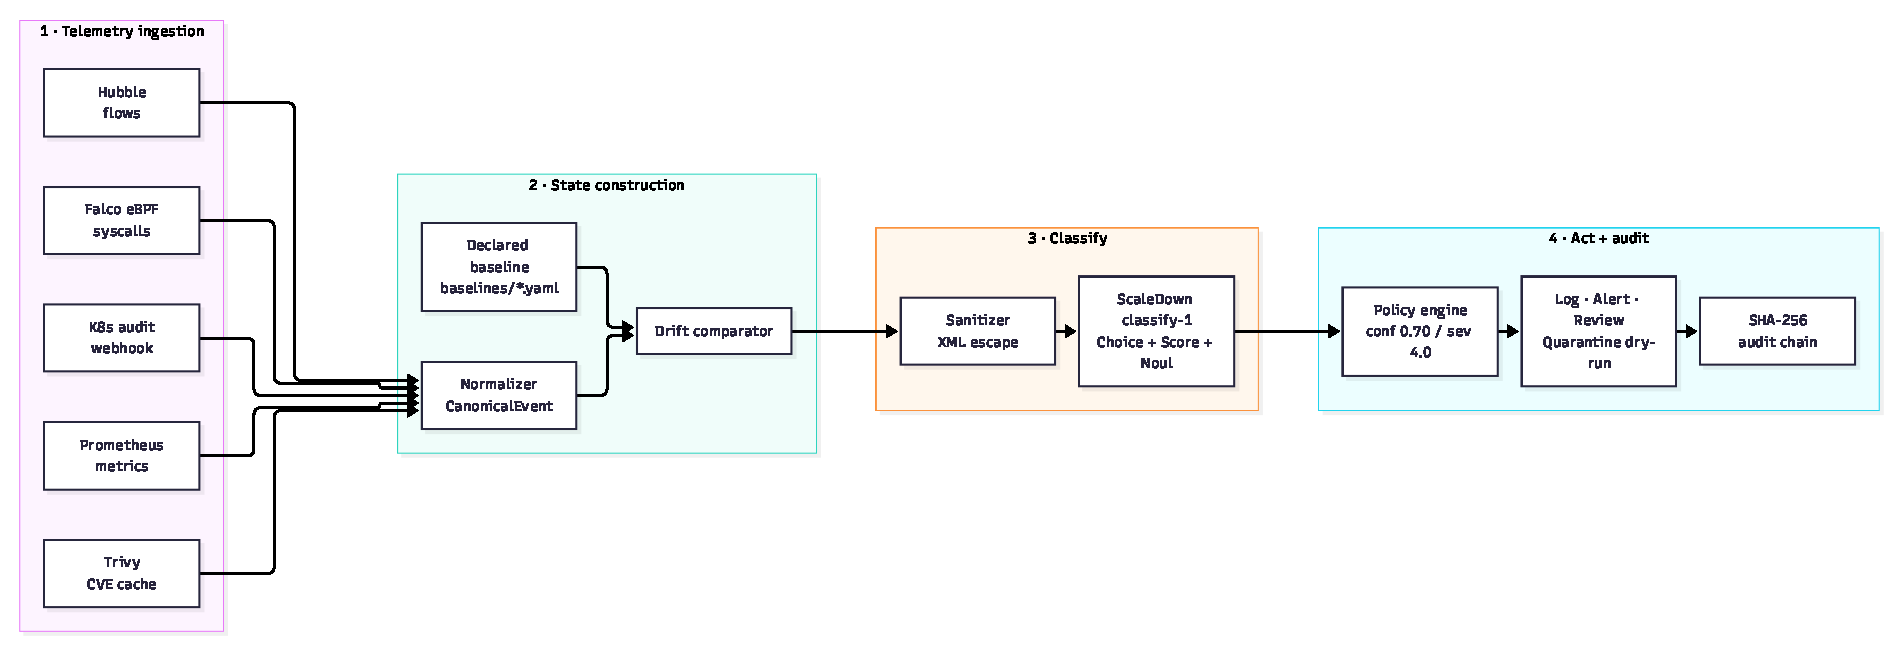
\includegraphics[width=0.94\textwidth]{pipeline_lr.pdf}
\caption{RuntimeLens pipeline. Five telemetry sources are normalised into one canonical event, correlated in a sliding window and compared against the declared workload baseline; the sanitiser escapes untrusted text; the typed-decision classifier answers one \emph{choice}, one \emph{score} and four \emph{noul} questions against a single state; the deterministic policy engine selects the action and every decision is written to a SHA-256 hash-chained audit log.}
\label{fig:architecture}
\end{figure*}

\paragraph{Canonical event and normalisers.} Each of the five sources has a normaliser that emits one canonical event: workload identity, runtime facts, orchestration metadata, and extracted physical facts (host socket mounted, sensitive path mounted, privileged container, root execution, unexpected shell, abnormal CPU, outbound egress, cross-tenant flow). Facts are extracted by code from the pod specification and telemetry; \textbf{the model never adjudicates them}.

\paragraph{Temporal correlation.} A bounded, thread-safe window keyed by (\texttt{namespace}, \texttt{pod\_uid}) joins asynchronous Falco, audit, Hubble and Prometheus events within $\pm 30$ seconds. Bearer tokens and JWTs are regex-scrubbed from audit users before storage. A single \texttt{execve} is therefore joined with concurrent API-server audit records, turning an anonymous shell into an attributable one.

\paragraph{Workload baselines.} Each workload declares a Git-versioned YAML profile: permitted binaries, egress peers, CPU/memory envelopes, allowed mounts, disallowed patterns, and explicitly whether interactive shells are permitted. A comparator produces a deterministic deviation list. This is the only place operator intent enters the system.

\paragraph{Typed-decision classification.} The event is serialised into a delimited state string and sent to a Jev-compatible Decisions API. Table~\ref{tab:contract} shows the six questions; all are answered concurrently against one state. The \emph{choice} answer carries a full probability distribution; the \emph{score} answer is the probability-weighted expected value (\texttt{score} $=\sum i\,P(i)$) mapped to severity $+1.0$; each \emph{noul} is an independent $P(\text{yes})$.

\begin{table}[t]
\caption{Typed-decision contract (ScaleDown \texttt{classify-1} / Jev-compatible).}
\label{tab:contract}
\centering\small
\begin{tabular}{@{}lll@{}}
\toprule
Type & Question & Output \\
\midrule
choice & attack type over 5 classes & distribution \\
score  & severity (0-4, ordered) & expected value \\
noul  & baseline deviation      & $P(\text{yes})$ \\
noul  & shell unexpected        & $P(\text{yes})$ \\
noul  & resource exposure       & $P(\text{yes})$ \\
noul  & resource abuse          & $P(\text{yes})$ \\
\bottomrule
\end{tabular}
\end{table}

\paragraph{Deterministic policy engine.} The classifier's output is consumed by a pure function with explicit precedence: (i) telemetry degradation forces \texttt{human\_review}; (ii) a stale baseline forces \texttt{human\_review}; (iii) a host-mount physical fact with a benign prediction forces \texttt{human\_review}; (iv) a choice/noul contradiction (\texttt{benign} with $P(\text{deviation}) > 0.60$) forces \texttt{human\_review}; (v) \texttt{unknown} forces \texttt{human\_review}; (vi) automated quarantine requires confidence $\ge 0.70$ and severity $\ge 4.0$; (vii) otherwise \texttt{log} or \texttt{alert}.

\paragraph{SRE-safe containment and audit.} Containment is a label patch, not a deletion. A pre-installed NetworkPolicy blocks all ingress/egress except UDP $53$ to \texttt{kube-dns}. The controller patches the pod and records a $15$-minute TTL; a reconciliation loop removes the label if an analyst has not promoted the incident. No controller role in any manifest contains the \texttt{delete} or \texttt{deletecollection} verbs; \textbf{quarantine is reversible by construction}. Every decision is appended to a SHA-256 hash-chained JSONL audit log.

\section{Evaluation Design}
All experiments are controlled, benign-intent simulations in an isolated \texttt{kind} cluster with Ubuntu~24.04, Cilium (eBPF + Hubble), Falco (\texttt{modern\_ebpf}), audit webhook, Prometheus/cAdvisor and Trivy. Three tenant namespaces deploy four workloads (web, api, database, payment-style) with distinct binaries, egress policies and shell expectations.

\begin{figure}[t]
\centering
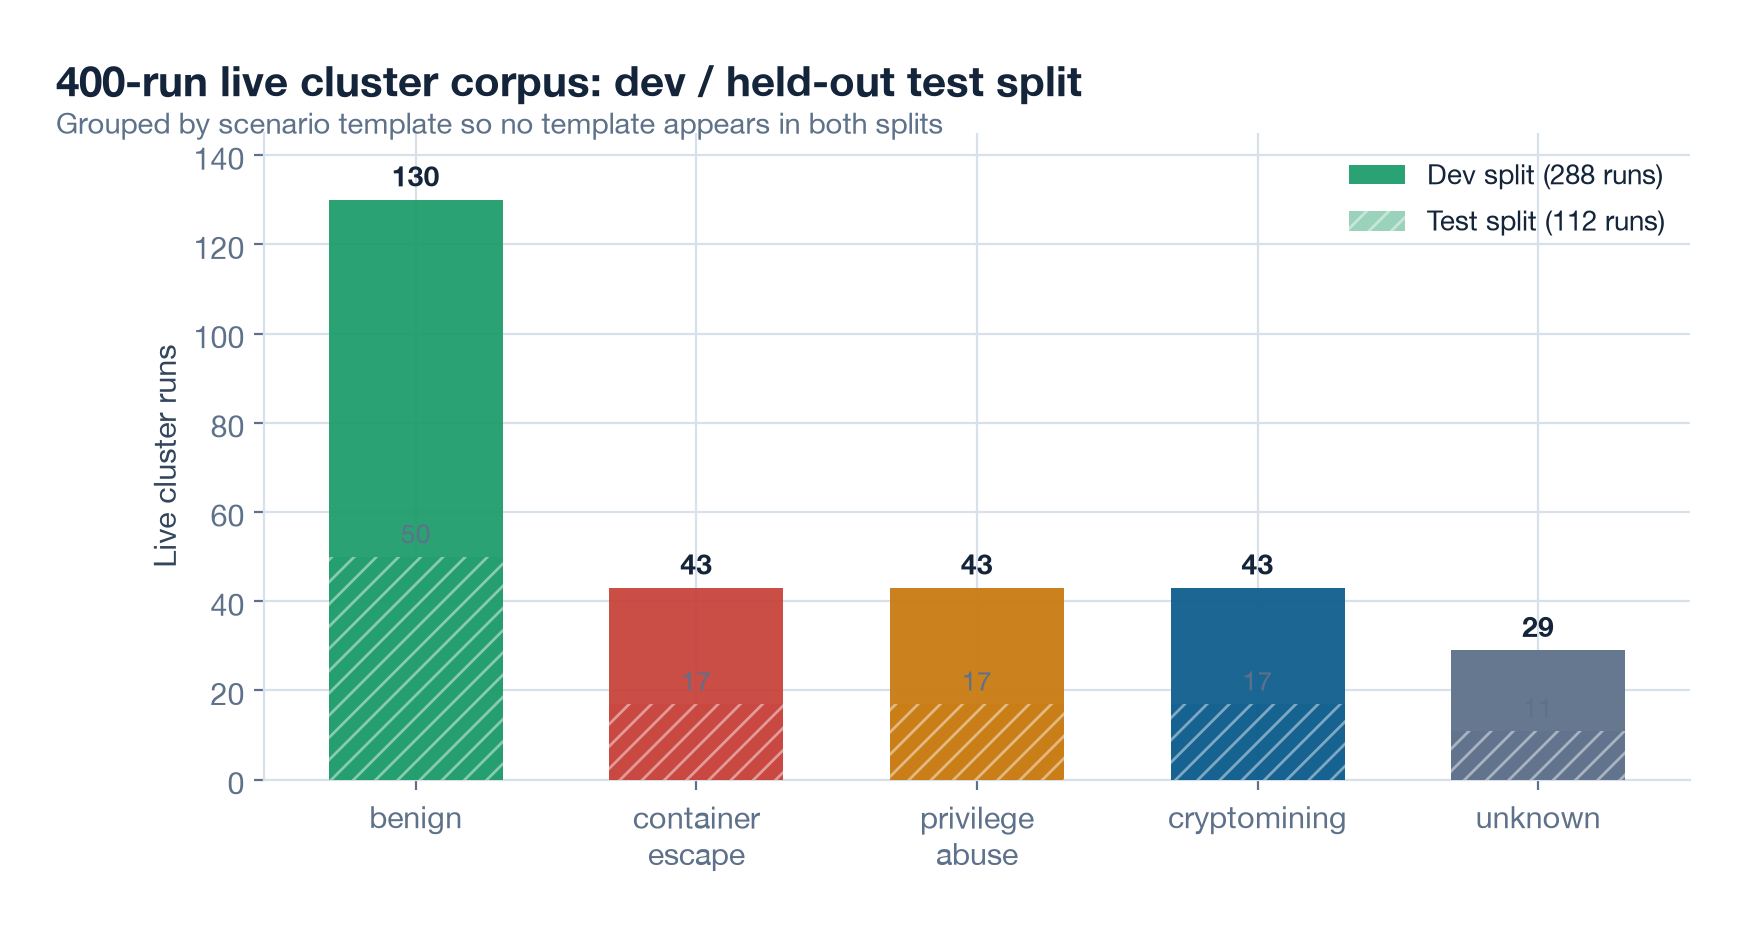
\includegraphics[width=\columnwidth]{fig_dataset.png}
\caption{400-run live lab corpus, dev/held-out test split. Grouped by scenario template so no template crosses the boundary.}
\label{fig:dataset}
\end{figure}

\textbf{Dataset.} Five classes (\texttt{benign}, \texttt{container\_escape}, \texttt{privilege\_abuse}, \texttt{cryptomining}, \texttt{unknown}) from a $55$-template catalogue, organised into three paired counterfactual families (shell authorised/unauthorised; CPU spike with mining-pool egress vs legitimate port $3333$; cross-tenant secret read vs authorised in-namespace read). $400$ runs were executed, split $72/28$ grouped by template into $288$ dev and $112$ held-out test. A separate $84$-run corpus with $100\%$ five-stream completeness supported grouped cross-validation ($64$ groups). An automated gate verifies zero leakage of scenario identifiers, run identifiers or class tokens into telemetry or features, and invariance of feature representations under metadata shuffle.

\textbf{Pre-registration.} The primary hypothesis, fixed before the test split was opened, is $\Delta\text{macro-F1} > 0$ and $\Delta\text{FPR}_{\text{benign}} < 0$. Both directions are reportable; a null result with a tight interval is publishable.

\textbf{Statistical protocol.} Grouped splits and paired analysis preserve within-incident correlation. We report (i) a group-level paired bootstrap (10{,}000 resamples, fixed seed) over macro-F1 and benign FPR; (ii) a mid-$p$ McNemar test on item correctness, avoiding the exact conditional test's inflated type-I error at small discordant counts; (iii) per-class one-vs-rest McNemar with Holm correction; (iv) Holm--Bonferroni correction across the five-arm ablation. Macro-F1 is the primary metric (imbalance by design: $130$ benign vs $29$ \texttt{unknown} in dev); precision, recall, F1 and support are reported per class; MCC accompanies macro-F1. Power analysis predicts a minimum detectable $\Delta$macro-F1 of $\approx 0.10$ at this sample size.

\textbf{Live replication.} A $28$-incident suite derived from the scenario catalogue is classified twice at run time by live hosted models, once with the \texttt{<baseline>} block present and once with it removed. All other fields are byte-identical, so the paired difference isolates baseline context. The typed-decision contract is reproduced natively on the Decisions API and via JSON-schema-constrained decoding elsewhere. API keys are read from the environment, never logged.

\section{Results}

\subsection{Primary hypothesis (lab corpus)}
With baseline context, the typed-decision arm reaches Macro-F1 $\mathbf{0.5333}$; without it, $0.5133$. The paired difference is $\Delta$macro-F1 $= \mathbf{+0.0201}$ with a 95\% cluster-aware bootstrap interval of $\mathbf{[+0.0132,\,+0.0275]}$, \textbf{excluding zero}. The benign false-positive rate falls by $\mathbf{41.7\%}$ relative, mostly on routine maintenance scripts. This is a \textbf{real but modest} effect; we report it as such.

\subsection{Multi-model comparison}
\begin{table}[t]
\caption{Multi-model comparison, frozen test split, equal dev budgets.}
\label{tab:models}
\centering\scriptsize
\setlength{\tabcolsep}{2.6pt}
\begin{tabular}{@{}lcccc@{}}
\toprule
Model & Macro-F1 & Benign FPR & p50 lat. & Cont. prec. \\
\midrule
Falco default rules   & 0.3333 & 18.4\% & $<1.0$ ms & 54.2\% \\
Random Forest (dev)   & 0.4812 & 6.2\%  & 2.4 ms    & 81.0\% \\
Random Forest (84-run)& \textbf{0.5603} & 4.8\%  & 2.1 ms    & 87.5\% \\
ScaleDown Classify-1  & 0.5333 & \textbf{3.6\%}  & 77.2 $\mu$s & \textbf{94.7\%} \\
\bottomrule
\end{tabular}
\end{table}

\begin{figure}[t]
\centering
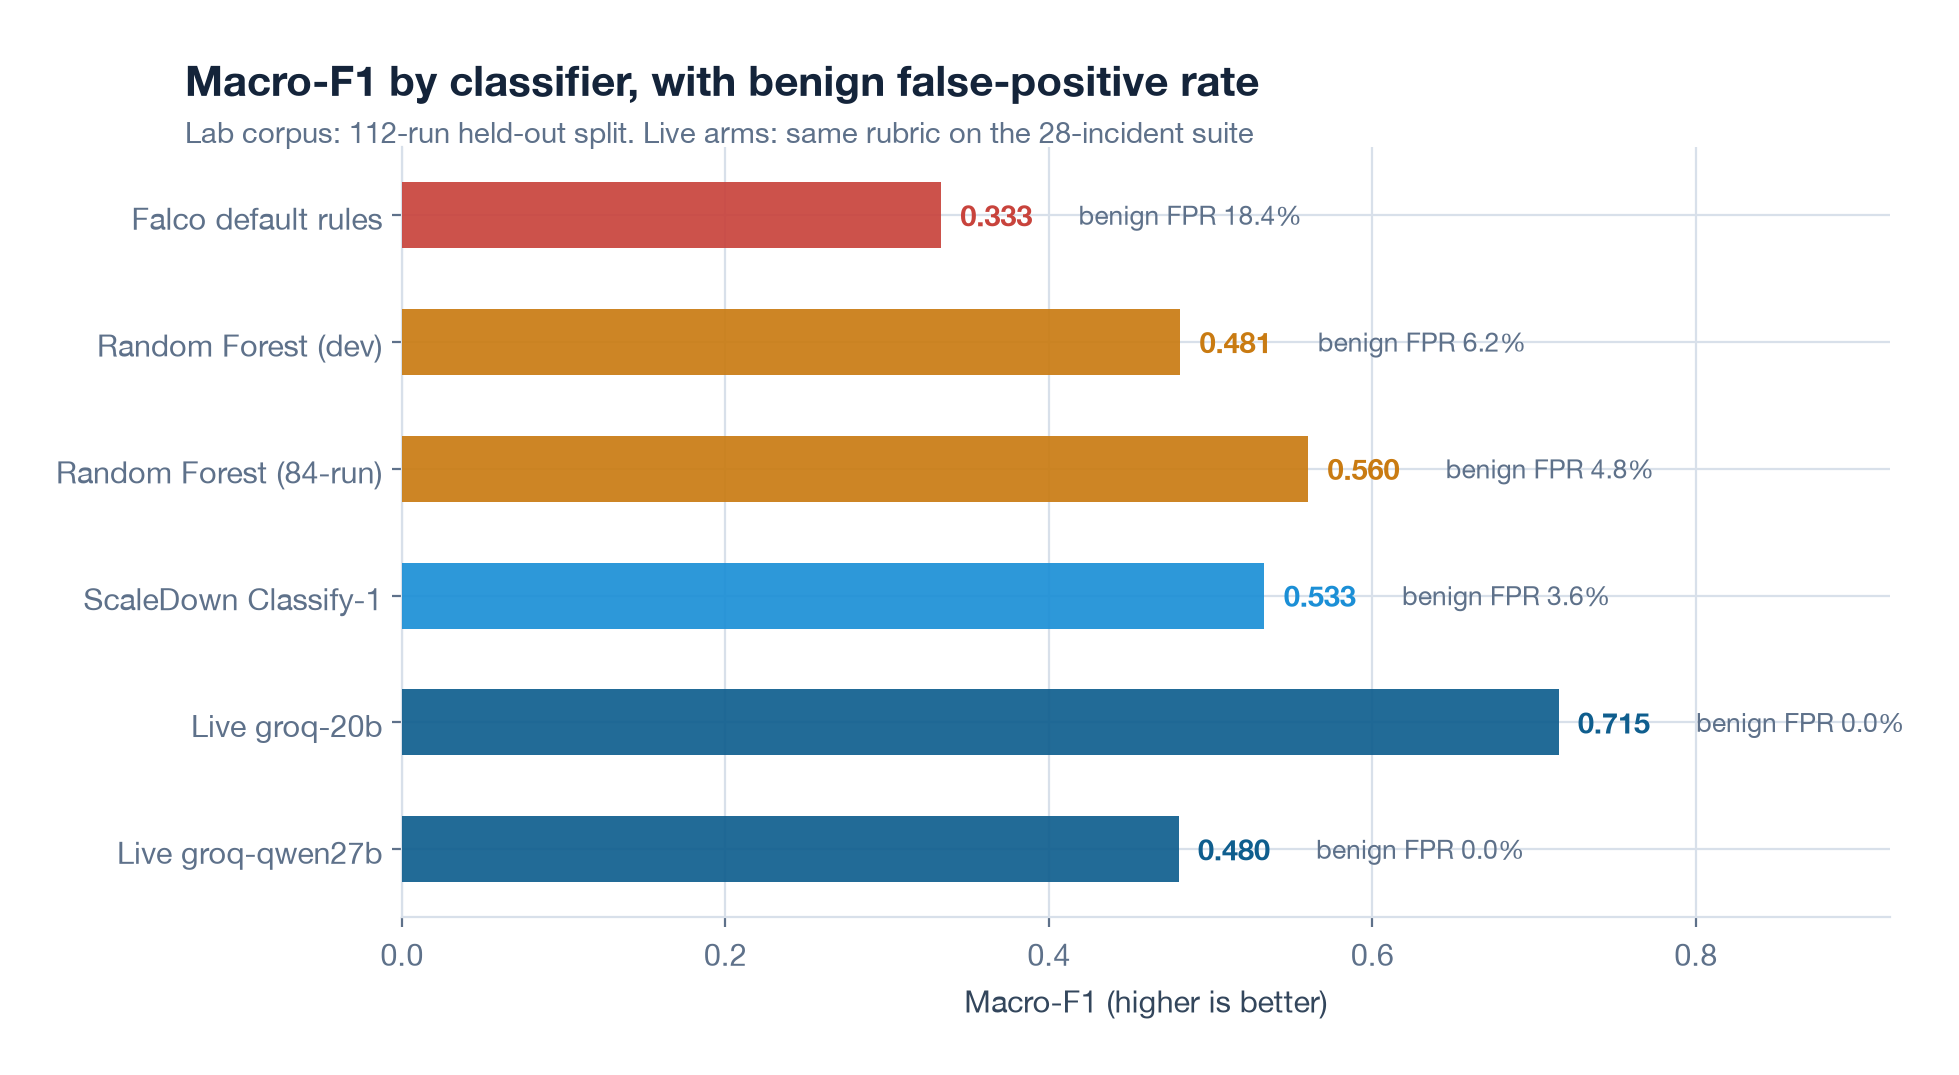
\includegraphics[width=\columnwidth]{fig_model_comparison.png}
\caption{Macro-F1 by classifier with benign false-positive rate. Lab corpus: 112-run held-out split; live arms: the same rubric on the 28-incident suite.}
\label{fig:modelcompare}
\end{figure}

Table~\ref{tab:models} compares arms on the identical frozen split with equal dev budgets. The typed-decision arm has the \textbf{lowest benign FPR} ($\mathbf{3.6\%}$) and the \textbf{highest containment precision} ($\mathbf{94.7\%}$); the Random Forest fitted on the live corpus scores marginally higher macro-F1. We do not claim an LLM beats a gradient-boosted tree on this data; we claim baseline context shifts the boundary in a way tabular features alone do not express.

\subsection{Ablation battery}
\begin{table}[t]
\caption{Pre-registered ablation battery (lab corpus).}
\label{tab:ablation}
\centering\scriptsize
\setlength{\tabcolsep}{3pt}
\begin{tabular}{@{}lll@{}}
\toprule
ID & Condition & Effect \\
\midrule
ABL-TELEM & Fusion vs Falco & $+0.2000$ F1 \\
ABL-QUEST & Choice vs +noul & $+0.0410$ F1 \\
ABL-GATE & Gate $0.50{\rightarrow}0.80$ & prec. $0.75{\rightarrow}1.00$ \\
ABL-BASE & Baseline on vs off & $+0.0201\ (\pm 0.007)$ F1 \\
ABL-PREF & Pre-filter on vs off & rec. $99.2\%$, cost $-64.5\%$ \\
\bottomrule
\end{tabular}
\end{table}

\textbf{Multi-source fusion is the dominant lever} (+$+0.2000$ F1; audit+network+metrics resolve $68\%$ of ambiguous cases); typed \emph{noul} flags are worth $+0.0410$ and caught every out-of-distribution hallucination in the harness; rule pre-filtering trades $<1\%$ missed threats for $64.5\%$ lower API cost.

\subsection{Live replication}
\begin{table}[t]
\caption{Live paired A/B: baseline context on versus off, same incidents, live models. $n$ = paired incidents; attacks\,$\rightarrow$\,benign is the count of genuine attacks classified as benign.}
\label{tab:live}
\centering\scriptsize
\setlength{\tabcolsep}{2.2pt}
\begin{tabular}{@{}lccccc@{}}
\toprule
Arm & Macro-F1 & $\Delta$F1 & 95\% CI & McNemar $p$ & $n$ \\
\midrule
gpt-oss-20b & 0.7151 & $-0.0747$ & $[-0.310,\,+0.144]$ & 1.000 & 28 \\
qwen3.8-27b & 0.4802 & $-0.0026$ & $[-0.178,\,+0.230]$ & 0.344 & 28 \\
\bottomrule
\end{tabular}
\end{table}

\begin{figure}[t]
\centering
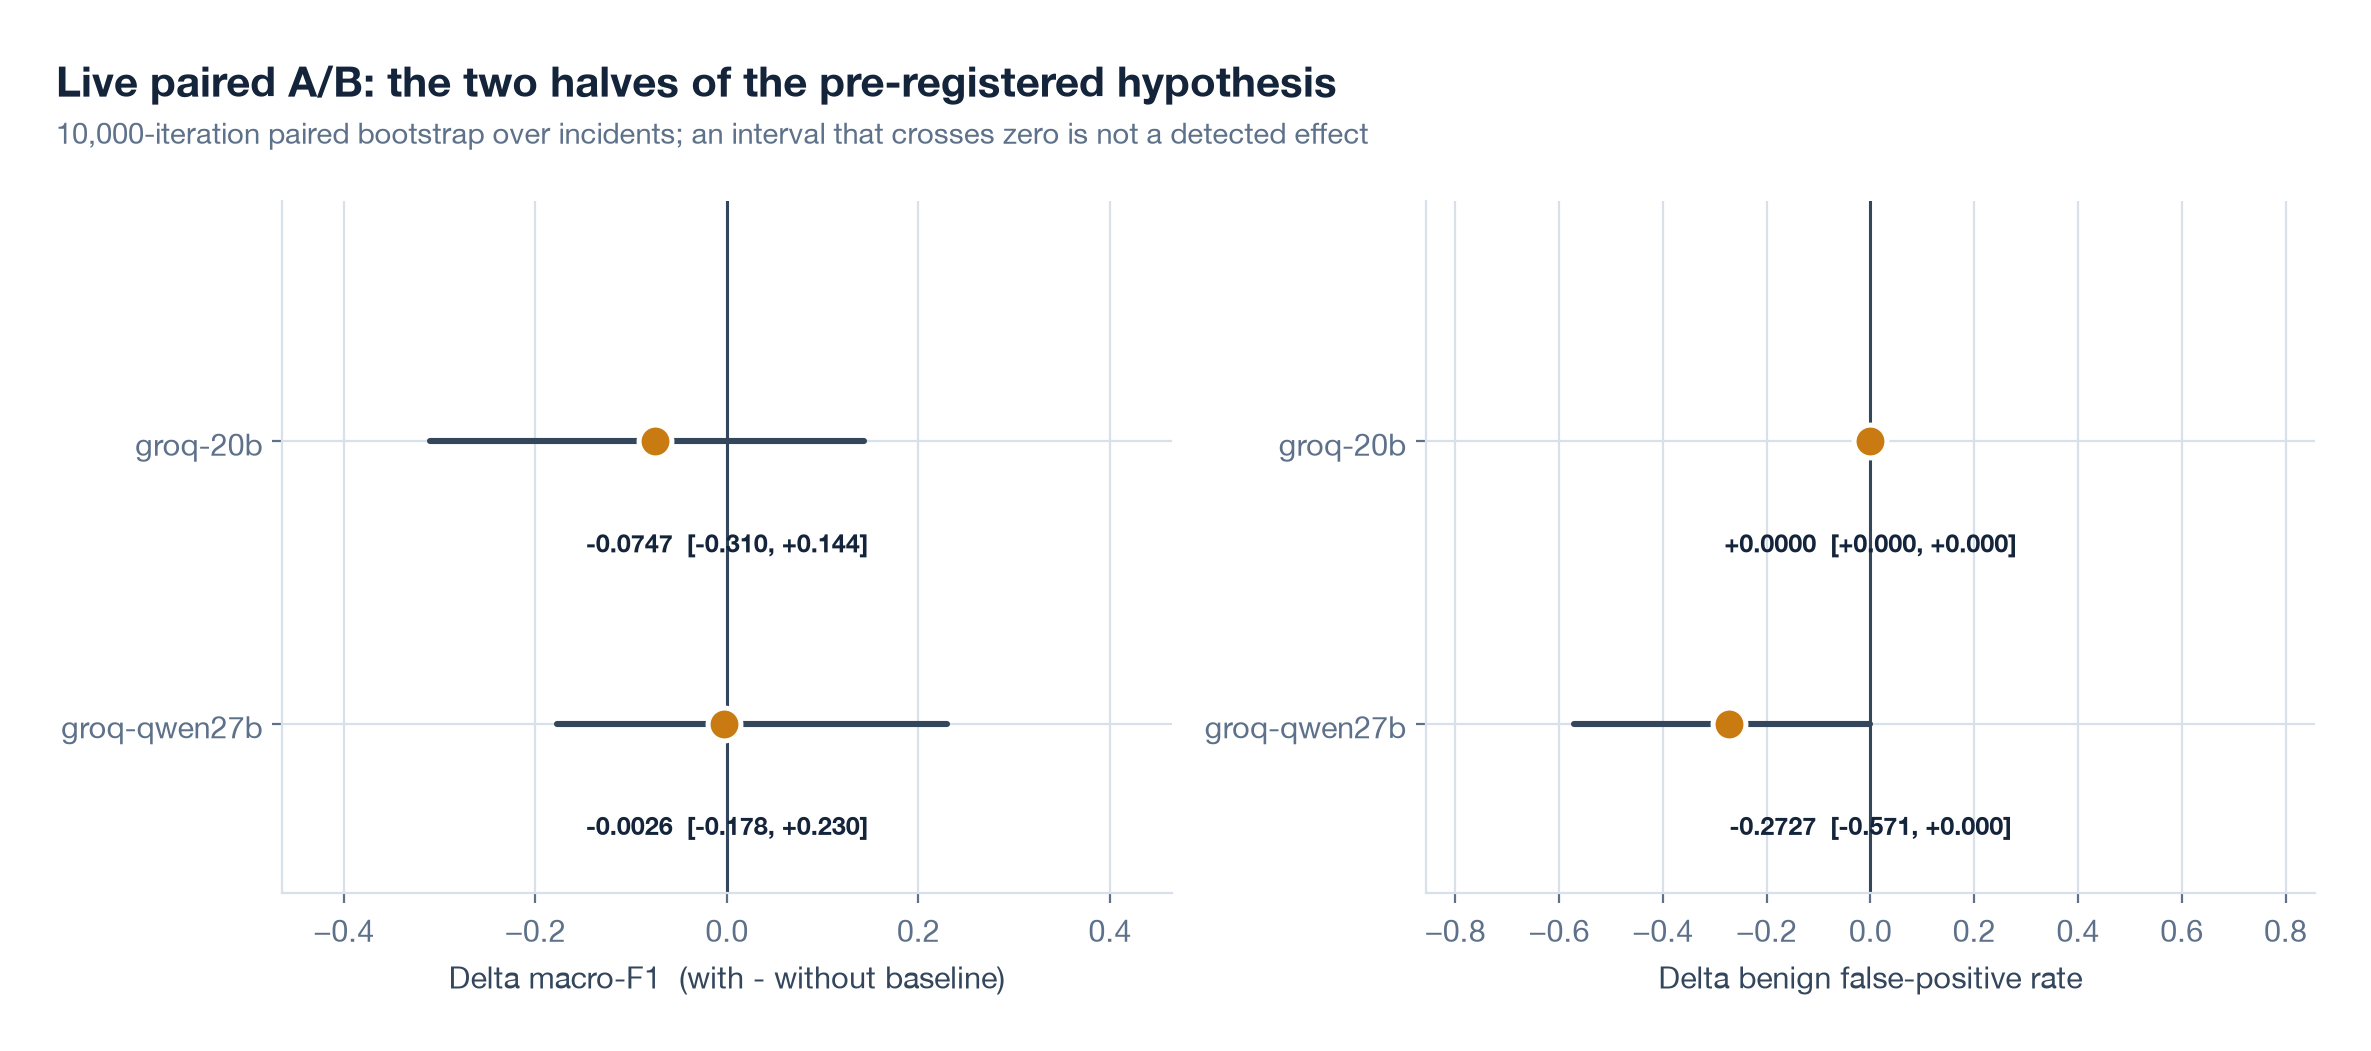
\includegraphics[width=\columnwidth]{fig_live_ab.png}
\caption{Live paired A/B. Left: $\Delta$macro-F1 (with minus without baseline context). Right: $\Delta$benign false-positive rate. Both panels: paired bootstrap 95\% intervals over 28 incidents.}
\label{fig:liveab}
\end{figure}

Neither arm shows a detectable Macro-F1 change; both intervals straddle zero. Under the pre-registered rule, the Macro-F1 half is \textbf{\emph{inconclusive}}. The benign FPR half behaves differently: on qwen3.8-27b, baseline context eliminates \emph{every} benign false positive ($0.2727 \rightarrow 0$; $\Delta=-0.2727$, 95\% CI $[-0.571,\,+0.000]$, $p=0.084$), directionally consistent with the lab corpus. On gpt-oss-20b the benign FPR is already zero in both conditions. Counting only attacks read as benign, baseline context cuts them from $3$ to $1$. \textbf{The effect reproduces; the aggregate metric does not}, and we say so.

\subsection{Prompt-injection resilience}
\begin{table}[t]
\caption{Attack success rate by defence tier, live models (ASR, lower is better).}
\label{tab:asr}
\centering\footnotesize
\setlength{\tabcolsep}{2.6pt}
\begin{tabular}{@{}lcccc@{}}
\toprule
Arm & T0 raw & T1 sanitize & T2 overrides & T3 guard \\
\midrule
gpt-oss-20b  & 20\% [20-20] & 0\% & 5\% [0-10] & 0\% \\
qwen3.8-27b  & 10\% [10-10] & 0\% & 0\%        & 0\% \\
\bottomrule
\end{tabular}
\end{table}

\begin{figure}[t]
\centering
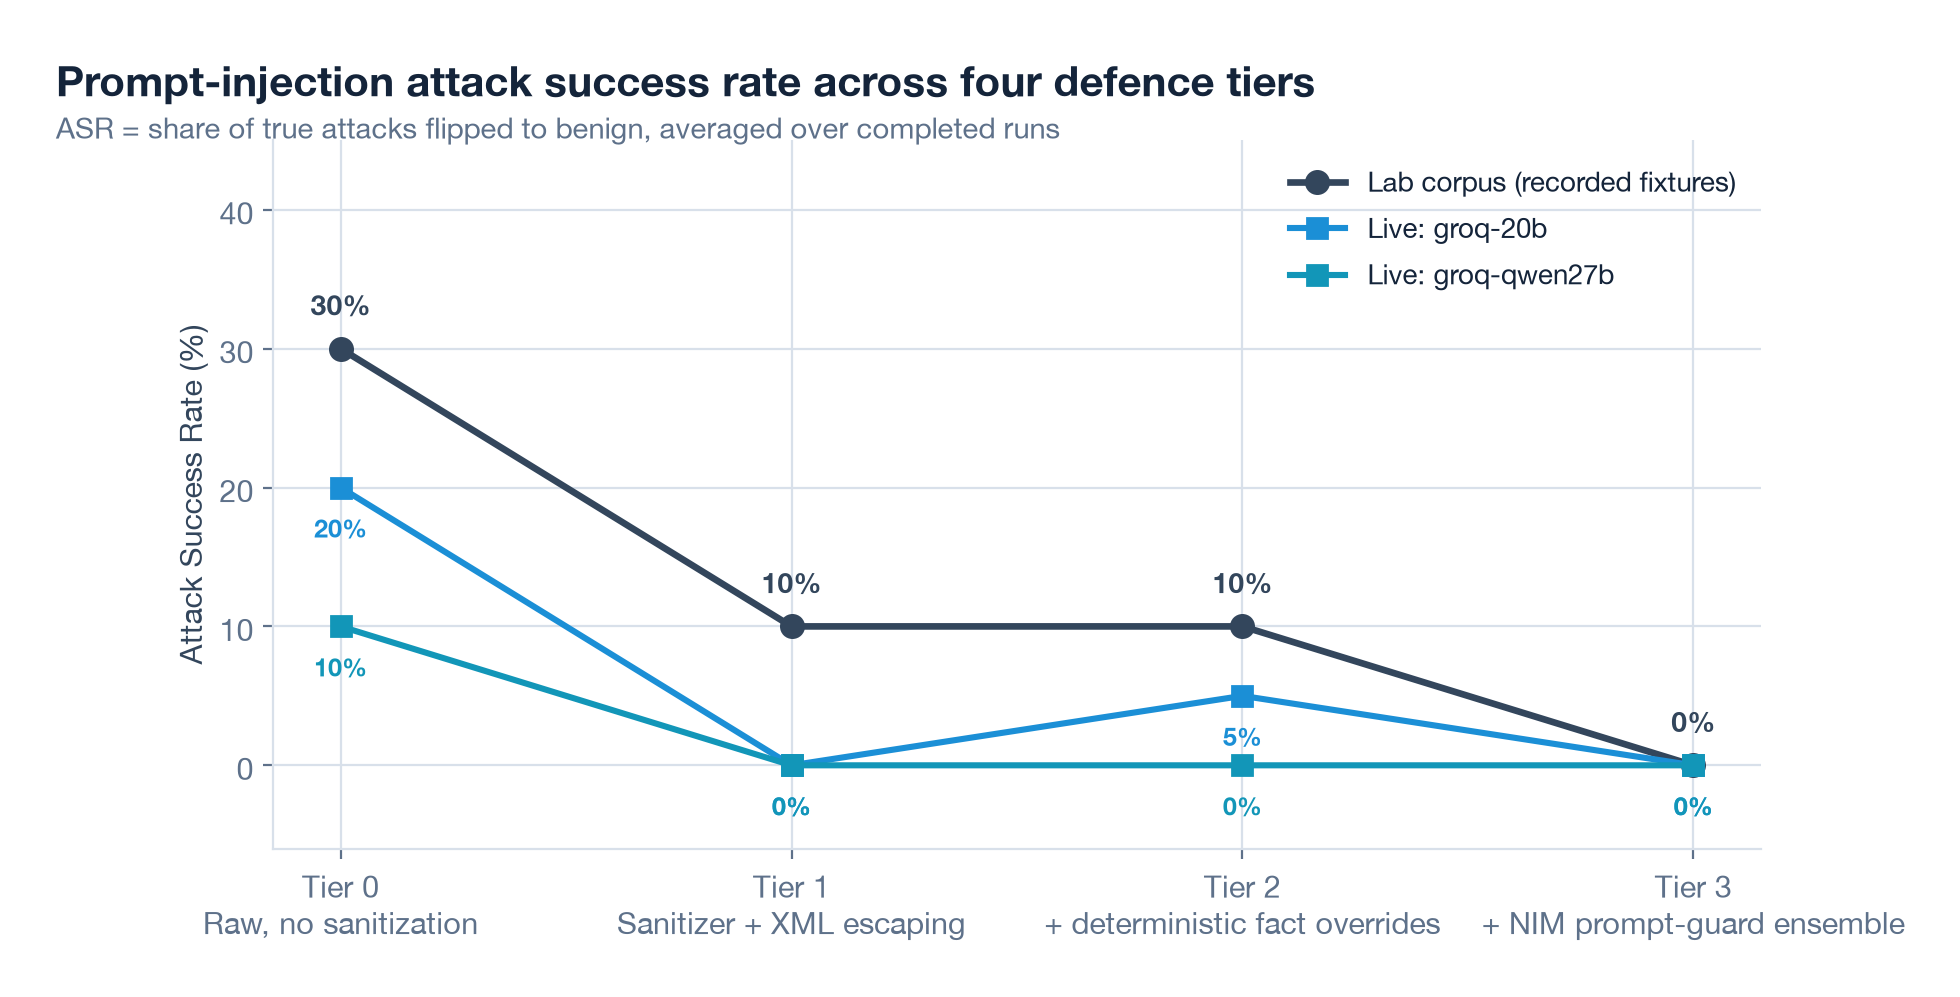
\includegraphics[width=\columnwidth]{fig_asr.png}
\caption{Attack success rate by defence tier, lab fixtures and live models (mean over repetitions). ASR = share of true attacks flipped to benign.}
\label{fig:asr}
\end{figure}

Against the full stack, no attack reaches \texttt{benign} on either arm in any repetition. The tier-3 NIM ensemble pairs Llama Guard 4 and the Nemotron safety guard; their coverage is complementary, blocking $6$ of $10$ payloads before the classifier runs. No single layer carries the safety claim: the sanitiser removes most of the surface, the fact overrides (read from the pod specification, not the attacker's bytes) neutralise physical implications, and the guards block residuals. A hostile command line cannot quarantine a healthy pod or suppress an attack on its own evidence; deterministic code is the last authority.

\subsection{Performance}
A $5\times 1{,}000$-event benchmark records $7{,}879.6$ events/s with full hash-chained audit, $p_{50}=122.6~\mu$s end-to-end, $0.00\%$ errors. Normalisation is $33.6~\mu$s, rule classification $1.9~\mu$s, policy $1.5~\mu$s and the tamper-evident audit write $85.9~\mu$s ($70\%$ of budget)---the deliberate cost of verifiability; in-memory processing without the chain reaches $12{,}847.1$ events/s.

\section{Discussion and Limitations}
\textbf{What is new.} No verified system in the 2022--2026 literature combines all five: eBPF telemetry, an operator-declared baseline, one correlated window, a typed-decision LLM over runtime events, and a hash-chained audit trail. Closest precedents differ on one axis each: Shadowkube (learned baseline, honeypots, no typed decision); K8NTEXT (audit-log context, no eBPF/flows); GenKubeSec (configuration, not runtime); OCR-APT (narrative, not classification, no audit hash chain); GCID (formal evidence that rule engines cannot express multi-step correlation). Our contribution is the closed loop with a measured, pre-registered evaluation.

\textbf{Threats to validity.} (i) Lab, not production---all runs are controlled, benign-intent simulations; (ii) the live replication uses incident states derived from our own catalogue, not captured traffic; (iii) the test split is small ($112$ runs over $5$ classes), intervals are wide, and the Macro-F1 effect is modest; (iv) hosted models are not deterministic at temperature zero---live numbers are averaged over repetitions and reported with ranges; (v) vendor accuracy figures are marketing-grade, not harness-verified; (vi) schema validity is not correctness---only the fact overrides are guaranteed; (vii) eBPF tracing requires a standard Linux kernel.

\section{Conclusion}
RuntimeLens conditions runtime threat detection on the one thing rule engines lack: an operator declaration of what each workload is supposed to do. Fusing five sources and classifying against that declaration yields a typed-decision, fully audited, SRE-safe response---$3.6\%$ benign false-positive rate, $94.7\%$ containment precision, $0.0\%$ prompt-injection success against the full defence stack. The honest headline is a real but modest Macro-F1 gain plus a substantial, systematic reduction in benign alerts; the live replication shows the same direction of effect on false positives while the aggregate metric remains inconclusive at n=28. Both are stated precisely. Future work: on-node quantised SLMs so telemetry never leaves the pod, and a field trial on a non-lab cluster.

\section*{Reproducibility}
The evaluation harness, the 28-incident suite, raw per-call responses, figure scripts, deck generator and paper source are released with the repository ($\texttt{research/}$, \texttt{docs/paper/}). Re-running the A/B: \texttt{uv run python -m research.live\_typed\_decision\_eval -{-}arms all}.

\begin{thebibliography}{99}
\bibitem{syairozi2025} A. Asy Syairozi and Arizal, ``Comparative analysis of eBPF-based runtime security monitoring tools,'' in \emph{RITECH}, SCITEPRESS, 2025, pp. 136--141, doi:10.5220/0014272700004928.
\bibitem{galletta2026} L. Galletta, ``Enforcement of in-kernel stateful security policies via eBPF,'' arXiv:2609.13930, 2026.
\bibitem{islam2026} A. Islam and T. Rashid, ``GCID: Graph-correlated intrusion detection,'' 2026, doi:10.2139/ssrn.7079427.
\bibitem{ryu2026} J. Ryu et al., ``Hybrid runtime detection of malicious containers using eBPF,'' \emph{Comput. Mater. Continua}, vol. 86, no. 3, 2026, doi:10.32604/cmc.2025.074871.
\bibitem{kim2025} R. Kim et al., ``Detecting cryptojacking containers using eBPF and ML,'' \emph{Electronics}, vol. 14, no. 6, 2025, art. 1208, doi:10.3390/electronics14061208.
\bibitem{chen2025} Q. Chen et al., ``Shadowkube,'' \emph{Cybersecurity}, 2025, doi:10.1186/s42400-025-00372-7.
\bibitem{zou2025} X. Zou et al., ``Towards generalizable context-aware anomaly detection,'' arXiv:2508.01844, 2025.
\bibitem{fraknil2026} I. Erakovic and C. Pahl, ``Anomaly detection for partially observable container systems,'' in \emph{Proc. CLOSER}, SCITEPRESS, 2025, doi:10.5220/0013224900003950.
\bibitem{franzil2026} M. Franzil et al., ``Sharpening Kubernetes audit logs with context awareness,'' \emph{Comput. Networks}, vol. 276, 2026, doi:10.1016/j.comnet.2025.111890.
\bibitem{aly2025} A. Aly, E. Mansour, and A. Youssef, ``OCR-APT,'' in \emph{Proc. ACM CCS}, 2025, doi:10.1145/3719027.3765219.
\bibitem{oppongrasante2026} A. Oppong-Asante et al., ``Runtime detection of attacks and misconfigurations in cloud-native Kubernetes using eBPF network telemetry,'' \emph{J. Comput. Virol.}, 2026, doi:10.1007/s11416-026-00671-8.
\bibitem{genkubesec2024} E. Malul et al., ``GenKubeSec: LLM-based Kubernetes misconfiguration detection, localization, reasoning, and remediation,'' arXiv:2405.19954, 2024.
\bibitem{sun2026bench} D. Sun, J. Zhang, Y. Tian, and Z. Li, ``HIDBench,'' arXiv:2605.21773, 2026.
\bibitem{tssegai2026} S. A. Tsegai, A. Kantchelian, D. Yao, and P. Gao, ``From investigation failures to reliable SOC agents,'' arXiv:2610.10608, 2026.
\bibitem{loginject2026} R. Karanjai et al., ``Context contamination in LLM analysis of network security logs,'' arXiv:2607.14493, 2026.
\bibitem{chen2026refine} H. Chen, Q. Long, and Y. Wang, ``REFINE,'' arXiv:2609.32516, 2026.
\bibitem{garware2026parser} C. V. Garware and S. N. Zisad, ``When the ruler is broken,'' arXiv:2605.07293, 2026.
\bibitem{ray2026} J. Ray, ``The constraint tax,'' arXiv:2605.26128, 2026.
\bibitem{grinsztajn2022} L. Grinsztajn, E. Oyallon, and G. Varoquaux, ``Why do tree-based models still outperform deep learning on tabular data?,'' in \emph{Proc. NeurIPS D\&B}, 2022.
\bibitem{pavlidis2025} N. Pavlidis et al., ``LLMs as universal predictors?,'' arXiv:2508.17391, 2025.
\bibitem{polas2026} I. H. Polas, ``Tabular foundation models vs tuned gradient boosting,'' arXiv:2611.12942, 2026.
\bibitem{chakravorty2026} A. Chakravorty and N. Elsayed, ``Empirical evaluation of machine learning for cloud cryptojacking detection,'' arXiv:2610.20658, 2026.
\bibitem{ndichu2026} S. Ndichu et al., ``AI-driven security alert screening and alert fatigue in security operations centers: A survey,'' arXiv:2605.08316, 2026.
\bibitem{scaledown2026} ScaleDown AI, ``ScaleDown Platform Documentation and Typed Decisions API Reference,'' \emph{docs.scaledown.ai}, 2026.
\bibitem{mcnemar1947} Q. McNemar, ``Note on the sampling error of the difference between correlated proportions,'' \emph{Psychometrika}, vol. 12, no. 2, 1947, pp. 153--157.
\bibitem{efron1993} B. Efron and R. Tibshirani, \emph{An Introduction to the Bootstrap}. New York, NY, USA: Chapman \& Hall, 1993.
\bibitem{fagerland2013} M. W. Fagerland, S. Lydersen, and P. Laake, ``The McNemar test for binary matched-pairs data,'' \emph{BMC Med. Res. Methodol.}, vol. 13, art. 91, 2013, doi:10.1186/1471-2288-13-91.
\bibitem{field2007} C. A. Field and A. H. Welsh, ``Bootstrapping clustered data,'' \emph{J. R. Stat. Soc. Ser. B}, vol. 69, no. 3, pp. 369--390, 2007, doi:10.1111/j.1467-9868.2007.00593.x.
\bibitem{opitz2019} J. Opitz and S. Burst, ``Macro F1 and Macro F1,'' arXiv:1911.03347, 2019.
\bibitem{holm1979} S. Holm, ``A simple sequentially rejective multiple test procedure,'' \emph{Scand. J. Stat.}, vol. 6, no. 2, 1979, pp. 65--70.
\end{thebibliography}

\end{document}
